\documentclass[11pt]{report}
\usepackage{fullpage}
\usepackage[pdftex,
            pdfauthor={Jeffrey Yoo Warren},
            pdftitle={Grassroots Mapping: a toolkit for participatory and activist cartography},
            pdfsubject={Participatory Cartography},
            pdfkeywords={Cartography},
            pdfproducer={Latex with hyperref},
            pdfcreator={pdflatex,colorlinks}]{hyperref}
\usepackage{graphicx,wrapfig,color,pdfcomment}
\definecolor{linkblue}{rgb}{0.2,0.2,1}
\hypersetup{colorlinks=true,
	    urlcolor=linkblue}

\title{Grassroots Mapping: a toolkit for participatory and politically engaged cartography}
\author{Jeffrey Warren}
\date{May 8, 2010}

%% Define a new 'jeff' style for the package that will use a smaller font.
\makeatletter
\def\url@jeffstyle{%
  \@ifundefined{selectfont}{\def\UrlFont{\sf}}{\def\UrlFont{\small\ttfamily}}}
\makeatother
%% Now actually use the newly defined style.
\urlstyle{jeff}

% Nadya's latex template:
% http://wiki.infosyncratic.nl/LaTeX

\begin{document}
\maketitle

\chapter{Introduction}
\section{Overview}
\section{Defining Grassroots Mapping: Toolkit, Practices, or Community?}

Exactly what makes up the Grassroots Mapping project? Is it a body of code, available under an MIT license at \url{http://github.com/jywarren/cartagen}? Is it a set of mapping practices, or tools, which have been employed in Lima, Peru, or Rio de Janiero? Or is it a community of practitioners and the web site, wiki, and mailing list which tie them together?

Fundamentally this project is intended to make the process of mapmaking easier for lay users, with the intent to broaden participation in cartography. In most places, maps can be seen as a tool of the state and of industry to express control over world we live in. By simplifying the means to create maps, from the data gathering through the editing and publication of digital and print maps, the tools are designed to democratize cartography. In turn, it is hoped that the ability of a broader public to make maps at accessible costs will help to empower bottom-up cartographic activism and to circumvent the current power structure of mapmaking. 

The core of the Grassroots Mapping project is the \textbf{application} of a novel combination of technology to specific communities. The technology consisted of low-cost aerial imaging with balloons and kites, and a novel online tool for stitching the resulting imagery into maps. The success of these tools is due to the effort and faith of the organizations and individuals who were willing to adopt these new and strange tools, and who saw their potential for use in the communities in Lima, Peru, and the oil spill crisis on the coast of the Gulf of Mexico. This includes Carla del Carpio of Manzanita "A" and Ernesto Fernandez of CEDRO, both in Lima, Peru, and Daniel Miracle and others from Escuelab, also in Lima. It includes Kris Ansin, Shannon Dosemagen, and Anne Rolfes of the Louisiana Bucket Brigade in New Orleans. It also includes the dozens of participants who tirelessly flew kites and balloons, and untangled and wound miles of string day after day. Perhaps most importantly, the tools grew and evolved in response to sustained use by participants, and with the input and collaboration of those who used them.

\subsection{Grassroots Mapping as Pedagogy}

To make this widespread adoption possible, the project also evolved to include a variety of teaching materials, printed guides, online videos, and workshops, both by the author and by the diverse collaborators who took ownership of the tools. These materials spanned a broad range of audiences, from 10-15 year old Spanish-speaking students to environmental activists in West Virginia and Kentucky. 

This documentation evolved as the author collaborated with and instructed participants in dozens of workshops over the past year. These occurred in diverse contexts, from a two week high school workshop at Beaver Country Day School in Chestnut Hill, outside of Boston, to an hour-long teaching session in City Park, New Orleans, for volunteers mapping the April 2010 BP Oil Spill. 

\subsection{Grassroots Mapping as a Community}

Ultimately, even the digital tools, including the Cartagen map rendering framework and the Cartagen Knitter, a tool for orthorectifying aerial imagery, were built with assistance and support of UROPs, colleagues, and contributors in the broader mapping community. That this has become the norm in technology projects does not detract from the fact that much of this work would have been impossible without such contributions. 

Building tools is unlike developing more abstract technologies in that to be successful, a series of compromises and pragmatic decisions must guide the design process, as well as continuous communication with an audience of users. The Grassroots Mapping project has evolved inresponse to these needs and should be examined in the context of the specific uses it has attempted to address, rather as an isolated or 'pure' work.

\section{Tools \& Technologies}

\subsection{Audience}

The tools developed as part of the Grassroots Mapping project address the needs of both committed enthusiasts who need powerful and efficient mapping technology, as well as those who have little experience and expertise but need simple and direct tools to make maps. Therefore, some of the tools, while being simple to use, are intended for 'power users' or those technically fluent in writing and editing code. The Cartagen framework falls under this category. Other tools, such as the balloon- and kite-based platforms for capturing aerial imagery, are intended for a wider audience, as is the Cartagen Knitter, a specific use of the Cartagen framework. A description of the various tools follows.

\subsection{Software}

\subsubsection{Interfaces for participatory cartography}

This section focuses on the framing, intent, and audience of the tools. A technical discussion of the tools can be found in Chapter 8. 

\subsubsection{The Cartagen framework}
\subsubsection*{Rendering architecture}
\subsection{Hardware}
\subsubsection{Balloon Aerial Photography}
\subsubsection{Photography from Kites and Unmanned Aerial Vehicles}
\subsection{Practice, Community, Support structure}
\subsubsection{GrassrootsMapping.org}
\subsubsection*{The Grassroots Mapping Wiki}
\begin{wrapfigure}{r}{0.5\textwidth}
	\begin{flushright}
		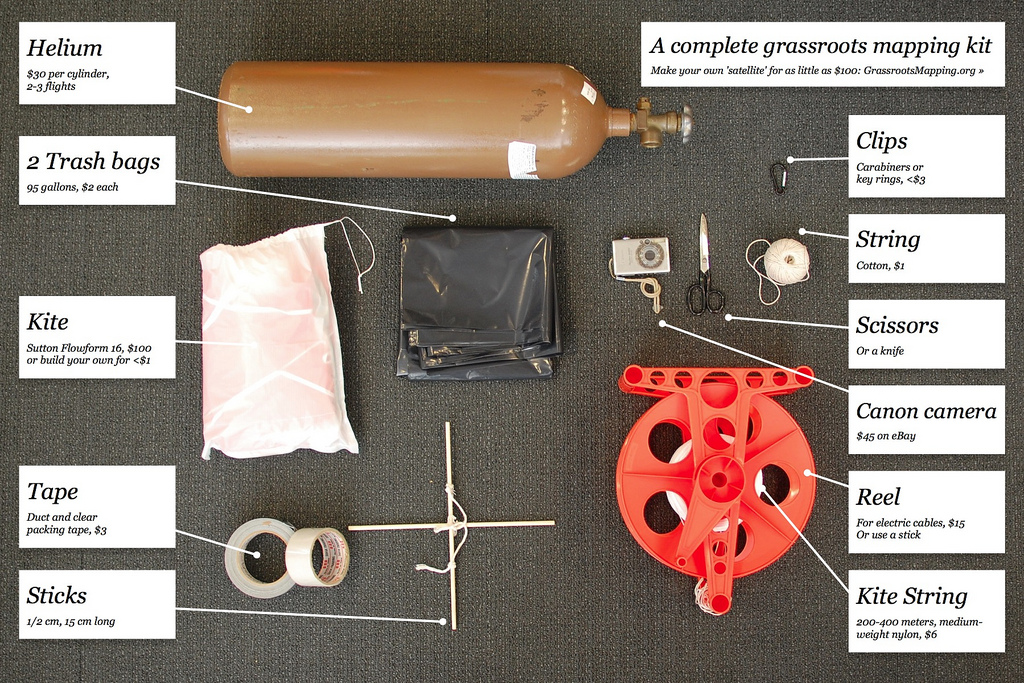
\includegraphics[width=0.45\textwidth]{images/100-dollar-satellite-poster.jpg}
	\end{flushright}
\end{wrapfigure}

\subsubsection*{Printed guides and support materials}
\subsubsection*{Curricular guides and teaching notes}

\subsubsection*{Documentation, case studies, Grassroots Map Collection}
\subsubsection*{The Grassroots Mapping community and mailing list}
\section{Novel Contributions}
\subsection{Novel application of low-cost tools to well-established need for raster imagery}
%\pdfcomment{do we discuss existing systems here? no, just mention paradigms of tiles, reference later section}

\subsection{Novel approaches to map rendering}
\subsection{Central merit: technology or culture?}
%both, duh: technology is only relevant in a context, and I make no attempt to separate this technology from its intended sociopolitical meaning

\chapter{Subjectivity in Mapping}

% text here, why is this chapter necessary:

The need for a more participatory cartography is predicated on the exclusion of many from the practice of map-making as it stands today. Even more importantly, it depends on the point of view that mapping is an inherently non-neutral practice, and that for maps to serve wider and more democratic interests, it must accommodate diverse viewpoints. Maps serve interests, and understanding their role not as documentation of what makes up the world, but as rhetorical, tactical, and \emph{subjective} tools is an important prerequisite to what this document argues.

\section{Neogeographers, Psychogeographers, and GIS}

A brief description of three distinct groups of practitioners is worthwhile, as each embodies a distinct conception of mapmaking. 

\subsection{Psychogeography}

\subsection{GIS practitioners}

Professional map makers have used Geographic Information Systems, or GIS since its development in the 

\subsection{Neogeography}

With the rise of web-based data and display systems came a group composed primarily of programmers and web designers, who have adopted the name \emph{neogeographers}. This group positions itself in contrast to 'traditional' approaches such as GIS, and 

% ... incomplete

Rana and Joliveau suggest that neogeography rejects the 'prescribed role/interaction between the four main components, namely the audience, the information, the presenter and the subject...'. 

% rana-joliveau-neogeography.pdf, 'NeoGeography: an extension of mainstream geography for everyone made by everyone?

% ... incomplete

Andrew Turner: Introduction to Neogeography
coined by Di-Ann Eisnor?
http://apb.directionsmag.com/archives/1379-Define-Neogeography.html

"outsiders"

\url{http://books.google.com/books?id=oHgDv4feV-8C&dq=neogeography+turner&printsec=frontcover&source=bn&hl=en&ei=gmDLS6_-KYj98AaY_KWXDA&sa=X&oi=book_result&ct=result&resnum=5&ved=0CBwQ6AEwBA#v=onepage&q&f=false}

"NeoGeography and the nature of geographic expertise", Author: Michael Goodchild  \url{http://www.informaworld.com/smpp/content~db=all~content=a911734343}
% goodchild-michael-neogeography.pdf

Orig. ref to Platial's usage: \url{http://placekraft.blogspot.com/2006/04/neogeography-defined.html}

% NEED reference for start of GIS practices 

\section{The mythical 'complete' map}

The most famous (yet fictional) version of this fantasy is Jorge Luis Borges' short story 

'a mile to the mile!'
'So we now use the country itself, as its own map, and I assure you it does nearly as well.' p.169

This idea was later elaborated in Jorge Luis Borges' 

% Of Exactitude in Science

% ...In that Empire, the craft of Cartography attained such Perfection that the Map of a Single province covered the space of an entire City, and the Map of the Empire itself an entire Province. In the course of Time, these Extensive maps were found somehow wanting, and so the College of Cartographers evolved a Map of the Empire that was of the same Scale as the Empire and that coincided with it point for point. Less attentive to the Study of Cartography, succeeding Generations came to judge a map of such Magnitude cumbersome, and, not without Irreverence, they abandoned it to the Rigours of sun and Rain. In the western Deserts, tattered Fragments of the Map are still to be found, Sheltering an occasional Beast or beggar; in the whole Nation, no other relic is left of the Discipline of Geography.

% From Travels of Praiseworthy Men (1658) by J. A. Suarez Miranda

% The piece was written by Jorge Luis Borges and Adolfo Bioy Casares. English translation quoted from J. L. Borges, A Universal History of Infamy, Penguin Books, London, 1975.

The idea that maps accurately, or even completely depict a location is not entertained in a literal sense, yet amongst

% Title: UK Motorways 100% Complete
% I'm pleased to announce that the main carriageways of all mainland UK motorways have been completed.  Over 3,000 km of roadway.
% Etienne Cherdlu Sat Jan 7 10:45:05 UTC 2006

\begin{wrapfigure}{r}{0.5\textwidth}
	\begin{flushright}
		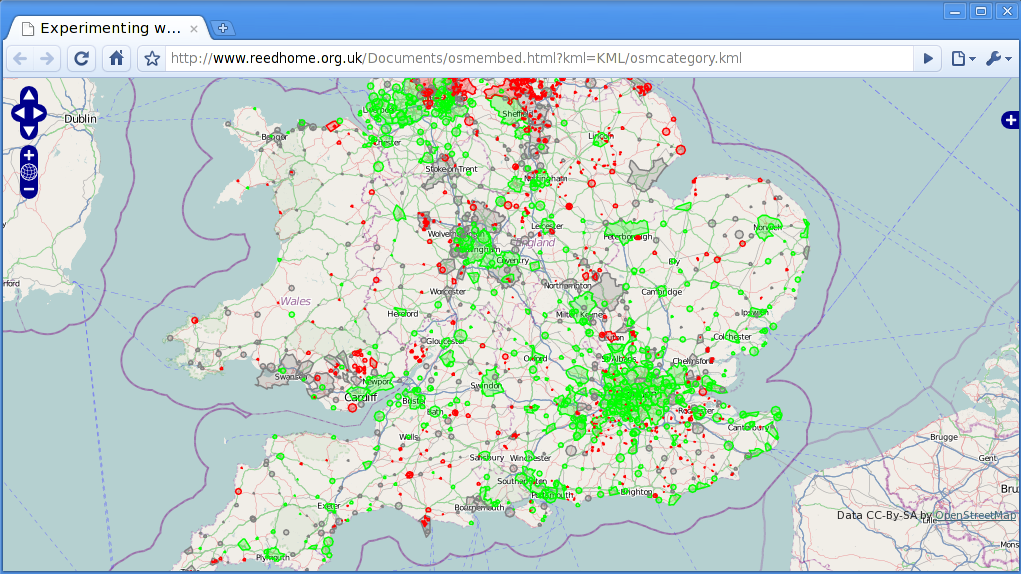
\includegraphics[width=0.45\textwidth]{images/osm-missing-parts.png}
	\url{http://www.reedhome.org.uk/Documents/osmembed.html?kml=KML/osmcategory.kml}
	\end{flushright}
\end{wrapfigure}

Chris Anderson 

%We often imagine 'complete maps'
% Epistomology and mapping: maps are a form of technology, and of power      
%  - OSM reference to a 'complete map of UK'
%        - Chris Anderson's Wired article of complete dataset
% "At the petabyte scale, information is not a matter of simple three- and four-dimensional taxonomy and order but of dimensionally agnostic statistics. It calls for an entirely different approach, one that requires us to lose the tether of data as something that can be visualized in its totality. It forces us to view data mathematically first and establish a context for it later."
% Read More http://www.wired.com/science/discoveries/magazine/16-07/pb_theory#ixzz0lTiRSTXp
% rebuttal: http://www.edge.org/documents/archive/edge248.html#hillis
\section{Maps as a 'window' onto the world}

% essentially epistemological issue.

For a variety of reasons, maps carry the weight of authority in a way that few other forms of evidence do; the main driver being the widely held belief that satellite or aerial maps are a kind of 'window' into the world. In photography the editorial role of the author is accepted, not to mention the damage which 'photoshopping' has inflicted on the perceived truth or even objectivity of the photographic image. Maps, however, continue to be taken as direct representations of reality, desipte the inherent subjectivity of image selection, color, brightness, and contrast processing, and the editorial eye necessary in reading and interpreting such imagery. 

\begin{wrapfigure}{r}{0.5\textwidth}
	\begin{flushright}
		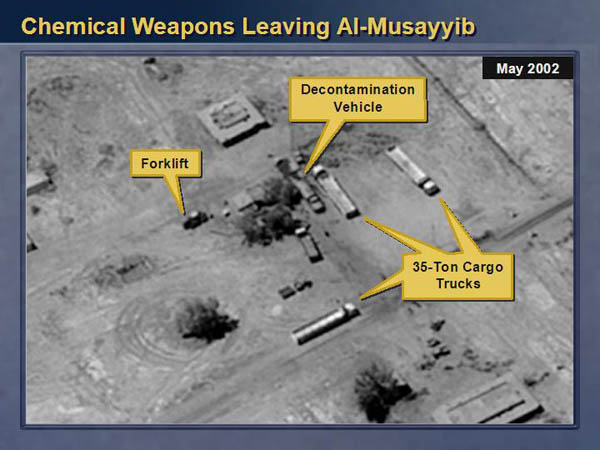
\includegraphics[width=0.45\textwidth]{images/iraq-image-16.jpg}
		\url{http://www.gwu.edu/~nsarchiv/NSAEBB/NSAEBB88/}, Image 16: Chemical weapons leaving Al-Musayyib
	\end{flushright}
\end{wrapfigure}

The best example of this attitude is of course the use of relatively low resolution satellite imagery by Colin Powell at the UN Security Council in February 2003, used as evidence to support the existence of weapons of mass destruction in Iraq. The subsequent complete absence of weapons did little to diminish the public's faith in such imagery as objective evidence. 
% citation http://www.un.org/apps/news/storyAr.asp?NewsID=6079&Cr=iraq&Cr1=inspect

\begin{quote}
``Let me say a word about satellite images before I show a couple. The photos that I am about to show you are sometimes hard for the average person to interpret, hard for me. The painstaking work of photo analysis takes experts with years and years of experience, pouring for hours and hours over light tables. But as I show you these images, I will try to capture and explain what they mean, what they indicate to our imagery specialists.

...

How do I know that? How can I say that? Let me give you a closer look. Look at the image on the left. On the left is a close-up of one of the four chemical bunkers. The two arrows indicate the presence of sure signs that the bunkers are storing chemical munitions. The arrow at the top that says security points to a facility that is the signature item for this kind of bunker. Inside that facility are special guards and special equipment to monitor any leakage that might come out of the bunker.

The truck you also see is a signature item. It's a decontamination vehicle in case something goes wrong."
	\cite{guardian2003powell}
\end{quote}

\begin{wrapfigure}{r}{0.5\textwidth}
	\begin{flushright}
		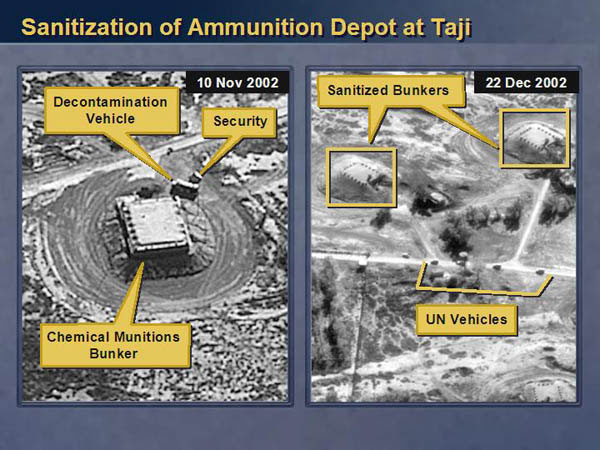
\includegraphics[width=0.45\textwidth]{images/iraq-image-13.jpg}
		\url{http://www.gwu.edu/~nsarchiv/NSAEBB/NSAEBB88/}, Image 13: Sanitization of Ammunition Dump at Tajii	
	\end{flushright}
\end{wrapfigure}

\begin{quote}
	``-- 10-11.***/WEAK. We support much of this discussion, but we note that decontamination vehicles--cited several times in the text--are water trucks that can have legitimate uses. A safer characterization is, `a vehicle used for chemical weapon decontamination.`

-- 11.***/WEAK. We agree there has been suspicious activity [redacted], including presence of a decontamination vehicle. We caution, however, that Iraq has given UNMOVIC what may be a plausible account for this activity--that this was an exercise involving the movement of conventional explosives; presence of a fire safety truck (water truck, which could also be used as a decontamination vehicle) is common in such an event."
	\cite{senate2004report}
\end{quote} 

% Fallacy!!! Wood, p. 20,21 - centimeter accuracy gives false impression of 'scientific accuracy' and completeness

What is most alarming about this kind of rhetorical use of map imagery is that it represents a means for those in a position of power to assert truths about places they have never been, without the involvement of human testimony from those who have.

This aspect of the public perception of maps as an objective, quantitative measure may have a relationship with the difficulty and expense of producing map imagery, and the traditional monopoly of government and high-tech industry in the production of such imagery.

\section{Maps: rhetorical, even tactical}
%        - Endless variety of possible data: Wood, Power of Maps, p.1
%        - not a representation of truth, but a rhetorical tool; Wood, p1?
%            - social construction of maps
% 	- map of sewer system from Wood
%	- Tactical cartography from Institute for Applied Autonomy
%	- http://www.tacticaltech.org/mapsforadvocacy
\section{Ground Truth, or maps as testimony}
%    - varying definitions of ownership, contested terrain
%        - 'Ground Truth' policy in OSM (http://wiki.openstreetmap.org/wiki/Disputes#On_the_Ground_Rule)

\section{Cartographic ethics}

In light of this reassessment of the political and social roles of maps and their production, some from the PGIS community have called for a code of ethics in participatory mapping projects. This seems especially prudent given that the production of maps can have dramatic effects on the residents of the mapped area. Giacomo Rambaldi, Robert Chambers, Mike McCall, and Jefferson Fox proposed in 2006 a set of 33 guidelines entitled "Practical ethics for PGIS practitioners, facilitators, technology intermediaries and researchers". The following is a sampling:

\begin{quote}
- Do your best to recognise that you are working with socially differentiated communities and that your presence will not be politically neutral
- Consider using spatial information technologies that can be mastered by local people (or local technology intermediaries) after being provided sufficient training
- Be considerate in taking peoples' time
- Stimulate spatial learning and information generation rather than mere data extraction for outsider’s analysis and interpretation
- Ensure that the outputs of the mapping process are understood by all those concerned
\cite{rambaldi2006practical}
\end{quote}

These guidelines demonstrate an belief that maps should be produced \textbf{in collaboration with} local communities, and with respect for their needs and interests. They have proved invaluable to the author in formalizing and understanding his interactions with mapping participants. In particular, they address the core concern of who owns the maps and for whom they are made; there is often the implicit assumption by enthusiasts of open geodata that simply dumping map data into OpenStreetMap is the end goal. It is important to be aware that most people (and especially those in communities in geographic conflict) are unaware of the existence of OpenStreetMap, and would likely be unreceptive to its benefits. 

Robert Chambers in particular warns PGIS practitioners against raising expectations of concrete results, noting that ``Any process of analysis facilitated by an outsider is liable to raise expectations of some benefit, even when the outsider goes to pains to explain that they have nothing to offer and nothing will follow from their visit. Disappointment, and reinforced disillusion with visitors and organisations outside the community then follow."


% email exchange from PPGIS list from early June 

% THIS WHOLE SECTION SHOULD PERHAPS BE MOVED TO 'DISCUSSION', post-Peru, or just after introducing state of the art... it may be a whole chapter.

Outline of history and benefits of PGIS, but also of ethics and beneficiaries

\subsection{Subjective cartography in practice}
%    - ref. West Bank mapping in Dec 2009
% Tree symbolism
% B'Tselem map of settlements
%        - mapping as testimony of use/presence/ownership by Abed's farm

\chapter{The Need for Geospatial Data}
\section{Two worlds of mapping}

Present-day users of web-based mapping products such as Google Maps are presented with an extremely rich cartographic landscape when they view maps of first-world urban centers such as New York and San Francisco. Real-time traffic data is often overlaid in lines of shifting red and green, and many buildings appear in orthographic '3D'. Well-known restaurants are interspersed with subway stops whose schedules may be called up with a few clicks. Routing algorithms offer turn-by-turn directions, optimized for pedestrians, bicyclists, and motorists. 

\begin{figure}[h]
	\begin{center}
		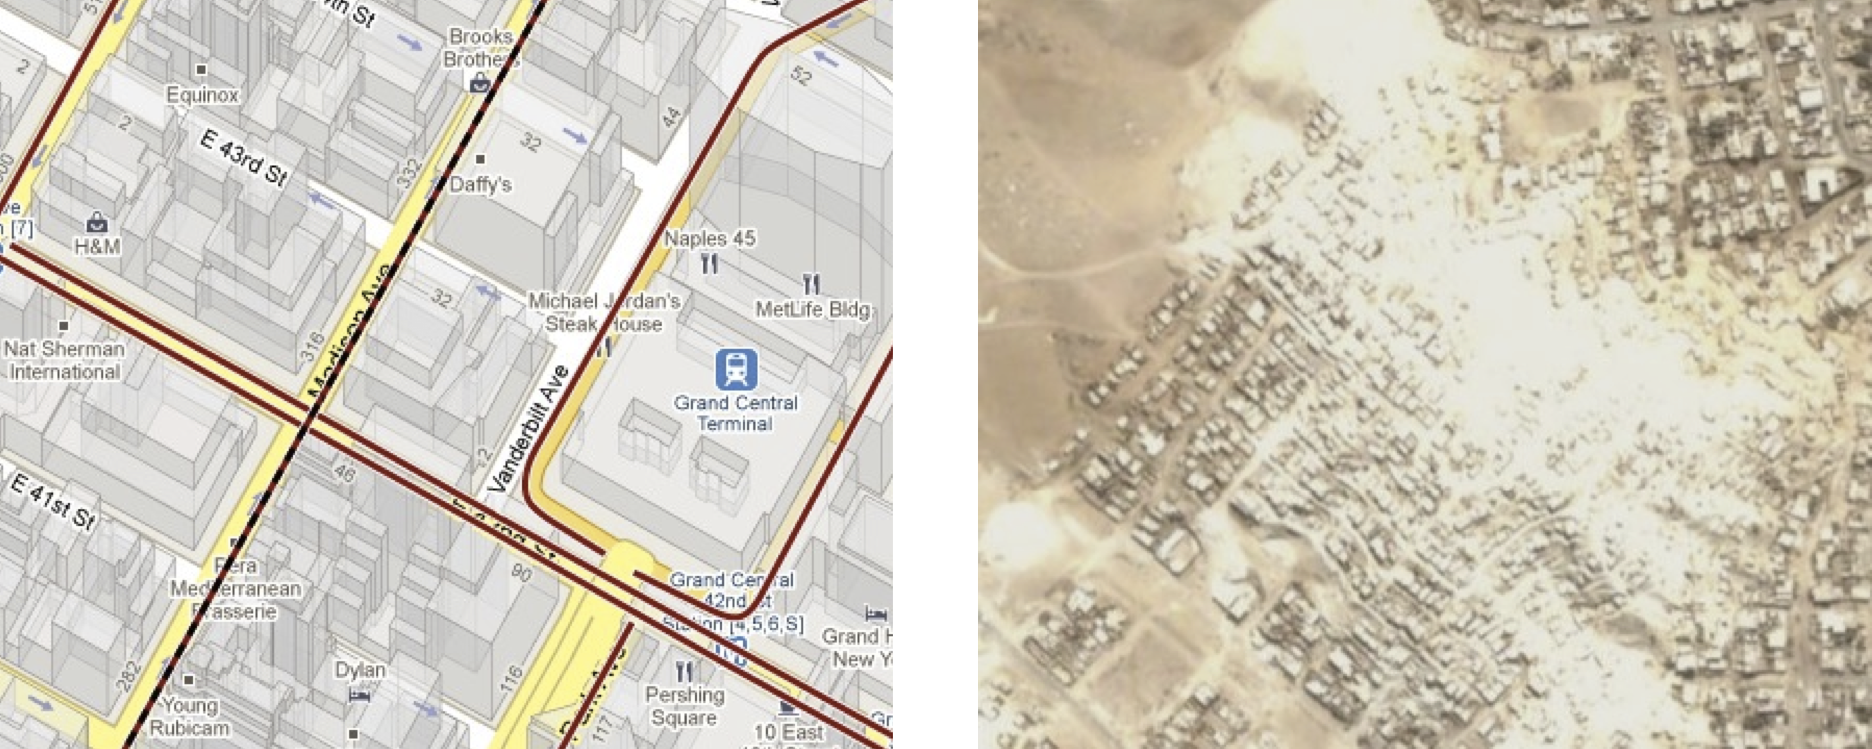
\includegraphics[width=1\textwidth]{images/two-worlds-mapping.png}
		Views of Manhattan, left, and a settlement in Lima, Peru, right, as seen in Google Maps \url{http://maps.google.com}
		% could add Cameroon, where towns are missing
	\end{center}
\end{figure}

Many are surprised when they view places such as Lima, Peru, a metropolis of 11 million people, and find that not far from the city center are vast areas of indistinct and unlabelled buildings. While some of these are recognized and official parts of the Municipality of Lima, many are informal settlements, whose inhabitants lack deeds to their plots of land, and whose streets and buildings do not appear on any city map. Many of these settlements, or 'invasions' as they are known to Peruvians, are governed by leaders who are either elected by the several hundred inhabitants, or who maintain control through intimidation -- employing thugs to collect taxes and enforce rules. 

A legal process exists to establish official land ownership in these settlements, and to issue deeds to their inhabitants, but the state lacks the resources to quantify or map these areas:

%    UN-HABITAT quotation
%	- “geographical mapping techniques to support struggles for social justice in India”. The end result, it added, could make maps as “tools to fight injustice in society”.
%	- http://timeoutbengaluru.net/aroundtown/aroundtown_feature_details.asp?code=59

In Lima, the organization in charge of land registrations, known as COFOPRI, requires residents to submit a plan -- essentially a measured and drawn map of their plots -- as one of many prerequisites to receiving a deed. Civil engineering firms have filled this gap by offering surveying and mapmaking services, but their high prices are a strain on the already poor inhabitants of the invasions.  

% find COFOPRI def
% image of posters showing what families owe to registration process

The Grassroots Mapping project was conceived as a means to broaden access to mapping technology, and was developed in direct response to the need for maps in informal settlements on the outskirts of Lima, Peru.

...

\subsection{Urban slums, informal settlements}

This state of affairs is not limited to Lima; by some estimates, a full quarter of the worlds population lives in urban slums. 

% find reference
% UN-HABITAT quotation

\subsection{Tenure mapping}

\subsubsection{The invasion of Lima, Peru}
%        - El Otro Sendero

The history of urban growth in Lima over the last hundred years can be described as a slow legitimization of vast areas of informal settlements; many populous and well-established districts such as Pamplona, Villa el Salvador and others, began as invasions decades ago.

Hernando de Soto, a well-known economist and champion of capitalism, ... quotation

Brief outline of fulfilled needs: chambers-who-empowered-disempowered-gains-loses.pdf, p.4
%            - graph of informal settlement percentages
%        - COFOPRI

\subsection{Mapping: a tool of empowerment or control?}

\begin{quote}
...it's frankly the same security through obscurity argument peddled for centuries, brought out most recently in Mumbai, a strategy on the verge of finally dissolving in a world of openness and transparency. The IDF access to much better intelligence and imagery than we'd ever have, they fly drones over Gaza, there's a 2m resolution commercial limit in all satellite imagery over Israel — guess who gets to see the sub-meter imagery? Gazans have nothing to gain by trying keep secrets, the asymmetry of that game is overwhelmingly not in their favor.\cite{maron2009misconceptions}
\end{quote}

\begin{quote}
In general, I view these edge cases as a question of power. Hiding information protects those already in power, but not those that are already marginalized. Legitimate cases to me is only information that puts dis-empowered people at risk, such as refugee routes along the Burmese-Indian border.\cite{maron2010freedom}
\end{quote}

Evgeny Morozov, "How dictators watch us on the web" - \url{http://www.prospectmagazine.co.uk/2009/11/how-dictators-watch-us-on-the-web/}
\url{http://irevolution.wordpress.com/2010/01/07/morozov-vs-shirky/} (Patrick Meier)

many criticisms may represent limited experience mapping... circular?
It is easy for activist cartographers who do not live in a community to advocate the use of tools which may put that community at risk.

"empowerment":(great article on definitions for empowerment and framework for discussing empowerment in the PGIS context)

Corbett, Jon M., and C. Peter Keller. 2005. An Analytical Framework to Examine Empowerment Associated with Participatory Geographic Information Systems (PGIS). Cartographica 40 (4):91-102.

\section{Environmental assessment}

Beyond issues of land rights and ownership, there are many other potential uses for inexpensive map data; the ability to produce photographic, or raster maps of sensitive environmental sites may empower small organizations which are unable to acquire timely or high resoultion satellite images of sites of interest. One case study we will examine is that of a group of environmental activists in West Virginia who have struggled to gather meaningful and quantitative evidence of the environmental damage and health hazards of mountaintop removal mining across the Appalachia region of the United States. Besides the prohibitive cost of traditional satellite imagery and high level of expertise required by traditional GIS tools, they strive for data which will make a visceral and emotional impact on policymakers and regulators, as well as the general public. 

Among other metrics, they make use of water conductivity tests to determine the degree of contamination due to runoff and blackwater releases. Conductivity is a secondary measure, and is not as direct as photography. Aerial imaging, or specifically mapping, is an ideal blend of direct measurement and visual appeal, and its main detractor is its price; overflights cost hundreds of dollars each and image processing is labor- and skills-intensive. A case study examining the applicability of Grassroots Mapping tools to this problem was performed in May 2010 and is discussed in Chapter 12.

\subsection{Asset allocation mapping and carbon cowboys}

\cite{poole2006there}

%	- bibliography/poole-peter.pdf
%	- stewardship of biodiversity, p.2
%	- case study uses of mapping capability, p.5
%	- detecting and monitoring impacts of industrial-scale development

\section{Open geodata and crisis mapping}
\subsection{Crisis mapping and Ushahidi}

A variety of different sorts of 'crowdsourced' or grassroots mapping strategies have evolved in recent years with the intent to respond to, document, analyze, and report on the real-time occurrence of disasters and crises. From environmental crises such as the April 2010 BP Oil Spill in the Gulf of Mexico to the humanitarian crisis in the aftermath of the January 2010 Haitian earthquake, a clear need has evolved for low-cost, decentralized situational awareness and documentation tools with geospatial features. Here we discuss some of the challenges of fulfilling such diverse needs under unpredictable conditions.

\subsubsection{Ushahidi}

The Ushahidi platform has emerged as a common and easy-to-install system for crowdsourced crisis reporting. Developed in collaboration with Kenyan programmers to help voters report election violence in Kenya in 200x, it allows citizens with mobile phones to send 140 character text messages to a publicized telephone number.\cite{okolloh2009ushahidi} These messages are read by a group of editors, who attempt to identify where the messages were sent from, and are published on a web site as red dots at their assumed location. That users self-report their locations, and can do so incorrectly, is tolerated because it may represent a means of privacy for users, and because in the aggregate it is quite difficult to 'fake' an event. Each report is 'verified' by ... 

% ref. AJ Turner's presentation at Where 2.0, i think - or Patrick Meier's on iRevolutioni
% interview LABB folks about how reports are verified

Ushahidi works in many cases because it is simple to understand on its surface; visitors to an Ushahidi web site see a series of dots with messages such as "I'm stuck under rubble" and imagine a person sending such a message from their cell phone. It makes use of existing communications infrastructure, namely that 'most people have cell phones' and relies on both a high level of literacy with text messaging and a willingness to send reports to a site which is not immediately viewable. However, it is not a means to 'make' a map, but rather to annotate an existing map with data points.

Ushahidi has been successfully used to gather and publish very up-to-date information about unfolding crises, for example in the instance created by the New Orleans-based environmental group Louisiana Bucket Brigade in response to the British Petroleum oil spill in April 2010. The kind of information it provides, however, is fundamentally difficult to verify or to quantify, and may be more useful in the context of emergency response than in evidence-gathering. Locations must often be approximated to the nearest town or city, and most reports are often just a few words with no name or photographic evidence. While geotagged photographs can be uploaded to Ushahidi, EXIF data can be falsified. In many cases there is an additional need for quantitative data. Map imagery provides better quality information in that every pixel of a map is georeferenced.  

\subsubsection{Photographs and maps as testimony}



\subsubsection{Satellite imagery access}

Public access to up-to-date imagery of crisis areas has become something of a hot-button issue in crisis mapping circles, as those companies and agencies in control of the imagery do not always elect to release it, or to license it freely for any use. Whethe due to an unwillingness to offer expensive imagery for unrestricted use, or due to the administrative burden of actually offering such data for download under a permissive license, access to satellite imagery has become a frequent bottleneck for aid organizations. 

Specifically in the bottom-up response to the Haitian earthquake and subsequent humanitarian crisis of January 2010, access became more difficult within weeks of the crisis. While GeoEye and other vendors generously offered open access to satellite imagery in the initial weeks of the crisis, most did not elect to do so on an ongoing basis, or for subsequent crises such as the February 2010 earthquake in Chile.



% Republishing Christiaan's response or UN-SPIDER's response may not be allowed, depending on the policies of the Crisis Mapping Network

% who released data??? 

Mikel Maron of the OpenStreetMap Humanitarian Team 

%	- origin in political mapping, focus on natural disaster
%        - UN-SPIDER/Google MapMaker response to Mikel Maron, Chile Earthquake

\chapter{State of the Art}
\section{PGIS: Participatory Geographic Information Systems}

Traditional GIS technology has been used for since the 1990's to support communities in developing contexts for purposes such as making tenure claims, environmental defense against petroleum and other extraction industries, as well as for planning purposes. This has become known as PGIS, or Participatory GIS, and typically... 

\begin{quote}
It was also in 1988 in an AKRSP (India) RRA training involving Jennifer McCracken, Anil Shah, Parmesh Shah and others, that a headman, asked to present to the villagers the map the outsiders had draw, had difficulty until he turned it ``upside down", which was the way he and the villagers saw their village . . . . We were teetering on the brink of learning that ``They can do it".
\cite{chambers2006participatory}
\end{quote}

% reference: Qualitative GIS book
% See Peter Poole's Life after Tenure Mapping for a brief historical timeline, i think

\subsection{PPGIS}

Definition: \url{http://www.ppgis.net/ppgis.htm}
Bibliography: \url{http://dusk2.geo.orst.edu/gis/student_bibs/slurie.htm}


bibliography/rambaldi-participatory-spatial-developing-countries.pdf

\subsection{Participatory GIS for Development}
% Jen Osha's article
%\href{http://www.directionsmag.com/article.php?article_id=2365&trv=1.}{Participatory GIS - A Paradigm Shift in Development?} - Jen Osha and Daniel Weiner, 2006
%        THE ILLUSTRATED GUIDE TO NONPROFIT GIS AND ONLINE MAPPING: http://maptogether.org/nonprofit-mapping
%        Claudia Canepa's PhD dissertation
\subsection{Shortcomings of traditional PGIS practice}
%    Peter Poole - Life after Tenure Mapping
%        - outsourcing of GIS processing typical, problems
\section{OpenStreetMap}

OpenStreetMap.org taken as an open-source software project, a database of open geodata, and a community of volunteer mappers, represents one of the best examples in recent years of the \textbf{neogeographic} response to PGIS. That is, without explicit ties to the PGIS movement, or even a high degree of literacy in the movements 2 decades of literature and research, OpenStreetMap (or OSM, as it has become known in neogeographic circles) has attempted to meet many of the same goals. OSM encourages volunteers around the world to contribute to a single, shared digital map and corresponding map database. 

In many ways it has met with wild success, and the size and detail of the OSM map database is formidable. 
% How big is it? 
However, participants are overwhelmingly European and American, and tend to be wealthy due to the emphasis on internet connectivity and the use of GPS devices to produce new map data.

In fact, the OSM data collection strategy relies most heavily upon three sources. First, existing municipal and public domain databases make up an enormous part of the available data; the TIGER database produced by the US Census increased the size of OSM by a factor of ten. Second, tracing of satellite data with the Potlatch, JOSM, and other tools to extract vector data from rasters plays a large role, especially in areas with few local participants. This technique was used in the Free Map Palestine project to map all of Gaza using a satellite dataset purchased for \$5,000 from donations during the Gaza war in late 2008. \cite{maron2010openstreetmap} While convenient in that it does not require mappers to actually travel to the places they are mapping, it does not actively involve residents of an area in the mapping process, and sufferes from many of the shortcomings which inspired the PGIS movement. 

Finally, much of the OMS database was created by individuals carrying GPS devices to record GPX tracks, or collections of latitude/longitude coordinates. These are later uploaded, annotated and merged into the main OSM database using tools such as JOSM. This is the preferred means of collecting data because of its high accuracy, its emphasis on firsthand mapping, the clear legal ownership of the data, and because of the implicit belief among many OSM participants that better maps are made `on the ground'. 

This belief is supported by the `on the ground' policy stated explicitly in the OpenStreetMap wiki, a central organizing document of the community.

\subsection{Humanitarian OSM Team}
 
An offshoot of the OpenStreetMap project known as the OpenStreetMap Humanitarian Team or HOT was started in late 2009 by Mikel Maron, a map programmer and co-founder of mapping firm Mapufacture. Positioned in direct response to the need for maps in areas of humanitarian crisis, Mikel has organized members from the technology community to visit crisis zones such as Port-au-Prince as well as a long-term presence in Kibera, a large slum in Nairobi, Kenya. HOT uses the same tools as the wider OpenStreetMap community, and either runs a separate instance of the OpenStreetMap server and database, or directly uploads the data to the main OpenStreetMap.org service. 

\subsubsection{Free Map Gaza}

%        Map Kibera, Free Map Palestine, Free Map India

Public domain data, JumpStart International

\subsubsection{Followup projects}
%        Data modeling: http://wiki.openstreetmap.org/wiki/Humanitarian_OSM_Tags/Humanitarian_Data_Model
\subsubsection{Challenges}
%        Slum mapping, disaster-specific issues
%        architectural/infrastructural shortcomings
%	reliance on GPS, or need for a base layer
% 	inclusion in a GPS-device process
%	ease of use, black-boxing of information
%	JOSM, other issues with typical deployment
\textbf{Emphasis on local infrastructure}

\section{Existing techniques for low-cost orthorectification}

While there are a diverse range of approaches to participatory mapping, several prior works have focused on free or widely available tools for orthorectifying aerial imagery as a means to produce and publish mapping data. Their uses range from stitching aerial imagery captured from hobby-levelremote control aircraft to rectifying historical printed maps in order to digitize their contents.

\subsection{Map Warper}

Perhaps the most ambitious project of this type is the Map Warper software written by Tim Waters, Schuyler Erle, and Shekhar Krishnan, as part of their project to 'crowdsource' the digitization of the New York Public Library map archive. \cite{waters2009warper} 

\subsection{GonzoEarth and manual stitching with Adobe Photoshop}

% mention DIYDrones, kite aerial photography guy with hugin/big Xs on the ground 

\chapter{Grassroots Mapping as an alternative means of participatory cartography}

How do the tools/technologies outlined above meet the needs described, and how are they better?

%    Meet subjectivity needs
%        - against a canonical datastore
%        - solution lays in tools and formats and practices, not in a single project/datastore
%            - therefore GM & Cartagen are based around:
%                - a body of code
%                - a thorough documentation and guide to mapping techniques
%		- a series of case studies
%        - options to organize project: as a 'generic hub' for imagery, like OpenAerialMap, engage primarily via internet/blogs
%            - or, focus on collaborating with specific communities in cartographic dispute
%                - expand into matchmaking between mappers and communities in need, as well as supporting via mailing list 
%                - maintain open communication with end-users, iterate back into tools: 
%                    - requests made via list: stewart long asks for masking, Crispen asks for entry of lat/lon pairs, WhereCamp folks asked for locking, Pat Coyle asked for 'natural_size' feature

\section{Aerial imaging with low-cost tools}

Due to the need for cheap and up-to-date imagery, a major part of the Grassroots Mapping project has been the design and use of low-cost platforms for capturing images of the ground from above. The use of kites and balloons to raise consumer-level 'point-and-shoot' cameras has allowed participants to capture images of sites of interest at minimal cost. A 'Grassroots Mapping Kit' can be assemnbled for less than \$100. 

\begin{quote}
In parallel came the discovery that local people could readily interpret black and white aerial photographs, often at 1:5000 (Dewees 1989; Mearns 1989; Sandford 1989). 
\cite{chambers2006participatory}
\end{quote}

\section{Cartagen: an alternative architecture for digital maps}

However, in order to orthorectify or `stitch' aerial imagery into a flat, geographically referenced map requires a system to display and manipulate raster imagery. The ability to label, trace, and otherwise annotate the resulting rectified map requires a system to display and manipulate vector data. In order to meet these needs the author created a map authoring and display framework called Cartagen. Written in JavaScript, it enables users to edit and publish discrete map data (points, lines, polygons) using a text editor, and to view and manipulate that data in a modern web browser such as Safari, Chrome, or Firefox. Maps may be published in just a few flat files, rather than relying upon a tile caching system or a backend database.

raster abilities of Cartagen

Beyond the ability to orthorectify imagery, Cartagen is a fully-fledged cartographic scripting environment and renderer. It can draw vector data onto a pixel grid - not just fast enough to generate tiles, but at over 10 frames per second on most computers. As the user interacts with a Cartagen map, features are drawn continuously, as in an animation. This negates the need to cache or otherwise store raster representations of map data, and sidesteps many of the assumptions and limitations of the modern mapping technology stack.

This alternative `geostack' is one of the most unique aspects of the Grassroots Mapping tool chain, but while some might see it as an unnecessary reinvention of the wheel,  

%        - existing solutions based around cloud systems
%            - this move opposite - closer to client
%            - needs: data under no connectivity
%            - multiple devices
%            - ownership of data/infrastructure
%                - FrontlineSMS, 'local' is a feature, opposite of corporate/commercial strategy
%        - low-AI approach; technical literacy, flexibility, admits 'misuse'
%            - examples: USGS overlay at WhereCamp 2010
%            - additon of non-map features with Warper tool
%            - difficulty of use of hugin, etc
%                - DIYDrones thread: "3 days stitching and tweaking images" (http://diydrones.com/profiles/blog/show?id=705844:BlogPost:134855&page=1#comments)
%            - Stewart Long uses Photoshop for most stitches (get him on record)
%Emphasis on building in response to end-user needs
%    - this work could only be done by working with communities in cartographic dispute. See Lima case study.

\chapter{Related works}
%    Inspiration, context, history of activist/grassroots mapping
%    Reiterate HOT/Free Map Palestine, India, Kibera
%    GroundTruth, Jai Sen, A People's Atlas of Chicago
\section{Beyond symbolic mapping: Data-driven approaches to participatory mapping}
%        Expanding role of mapping to legal, tactical
%        Institute for Applied Autonomy

\chapter{Evaluation criteria}
\section{Participants vs. collaborators}
%        Role of Carla, Escuelab, Shuawa
%        Hector as a fellow educator (interview)
%    'Reconceptualizing Validity' (Patti Lather, p.67)
\subsubsection{Triangulation}
\subsubsection{Construct validity}
how theory was affected by data
\subsubsection{Face validity}
how research was received by participants
\subsubsection{Catalytic Validity}
how participation transforms the situation (self-awareness/reflexivity)

\subsection{Interviews with local partners}
Wiki, mailing list, blog, media coverage (~ Face validity)

\chapter{The Grassroots Mapping tool chain}
\section{Balloon/kite Aerial Mapping (BAM/KAM)}
%    UAV - DIYDrones and collaboration (see 'Future work')
%        Leveraging both expert and 'amateur'/enthusiast expertise
%        Connecting hobby/DIY communities with activist communities and agendas
\subsection{Accuracy and precision in kite and balloon imaging}
% focus on cost goals, 'mapping at all'
% Eric Wolf's thesis on BAP metrics: wolf-eric-thesis.pdf

\section{Digital maps: reconceptualizing mapping interaction}
\subsection{Beyond raster mapping/Tile politics}
%            Metadata: authorship data
%            Google Maps png metadata hack
%            GIS and broadly adopted consumer-focused mapping stacks
\subsection{Cartagen dynamic rendering}
%            Existing vector systems (Chris Schmitt's email on geowanking)
%            Limitations: technical, barrier-to-entry, participatory, literacy
%                GSS (and OSM-JSON): appropriating the HTML/CSS paradigm for data legibility and open access
%                    Format politics: XML, JSON, RSS
\subsection{An iterative toolchain development process}
%    Toolchain not developed in vacuum, but through collaboration and study on-site
%        - initial flight testing with Josh Levinger
%            - MIT map
%            - terrain, difficulty
%            - optimization for site: Peru, low buildings, no trees
%        - Peru, West Bank, India
%        - Following chapters document those collaborations and their fruits
\subsection{Web-based orthorectification and warping}

In response to the collaborative design process and interviews conducted in Lima, Peru (Chapter 9), it was determined that the primary barrier to producing map imagery was the orthorectification process. While in Lima, participants made use of Adobe Photoshop CS3 as well as the Map Warper software developed by Tim Waters, Shekhar Krishnan, and Schuyler Erle. Attempts were made to instruct residents of the subject areas in the use of these tools. These techniques met with limited success due to factors such as availability of computers powerful enough to run Photoshop, latency in internet access, and most of all, the obscure interfaces which users were required to learn. Map Warper, which uses a ground control point (GCP) matching technique wherein users are asked to identify coordinates which appear in both a source image and a base reference map. 

% this may be redundant with related works or state of the art

\begin{wrapfigure}{r}{0.5\textwidth}
	\begin{flushright}
		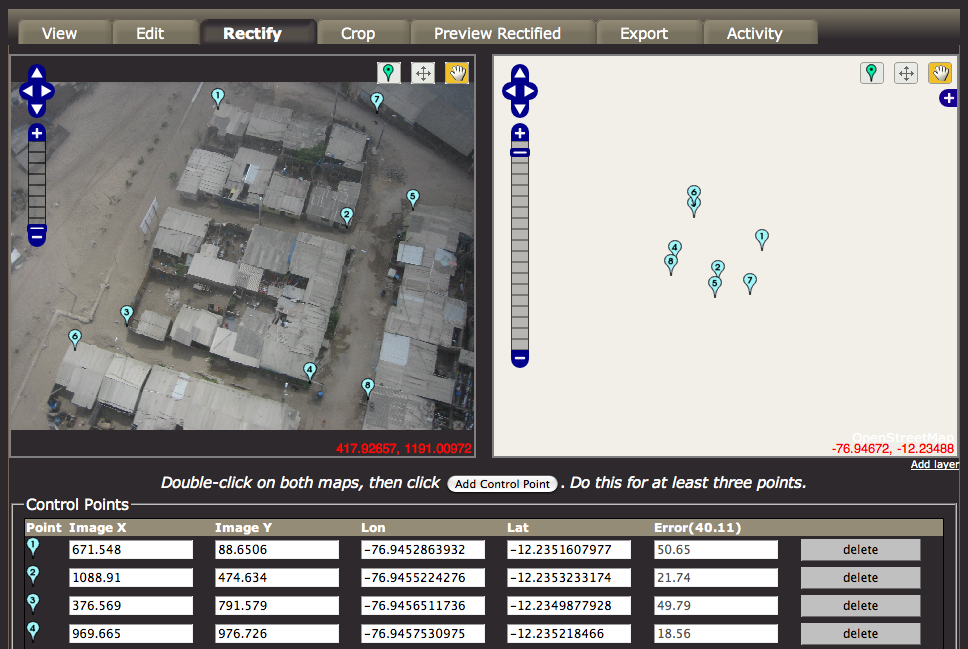
\includegraphics[width=0.45\textwidth]{images/map-warper.png}
		The Map Warper interface for identifying Ground Control Points. \cite{waters2009warper}
	\end{flushright}
\end{wrapfigure}

\begin{wrapfigure}{r}{0.5\textwidth}
	\begin{flushright}
		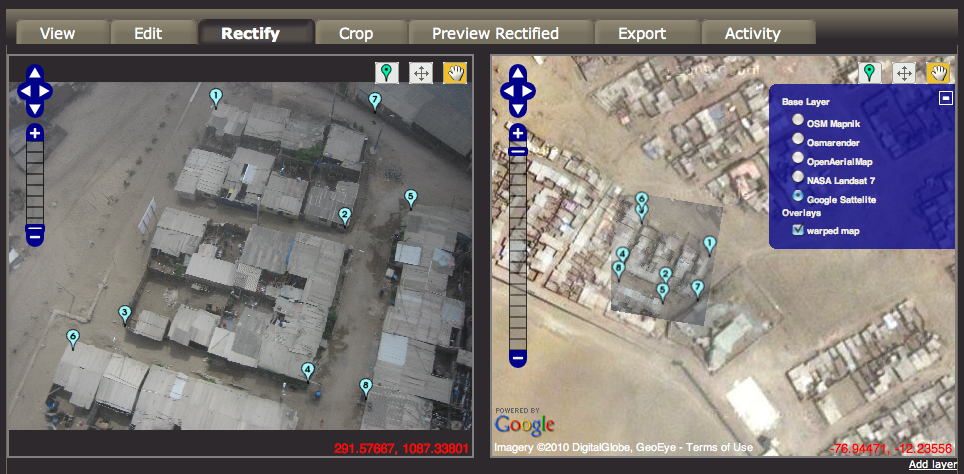
\includegraphics[width=0.45\textwidth]{images/map-warper-hack.png}
		Demonstration of JavaScript hack to insert Google satellite data for warping in areas with low feature density. \cite{waters2009warper}
	\end{flushright}
\end{wrapfigure}

Using Adobe Photoshop to manually disort and warp imagery over an imported base map was a more direct and easier to explain process, but the low availability of the software and the need for a powerful computer to perform large image transformations were additional challenges. The need for a lightweight, easy to use system became clear. The additional ability to run such a program in any standard web browser would put such tools within reach of anyone with access to an internet cafe.

The Cartagen Knitter software, developed in the months following the Lima, Peru mapping project, makes this possible. Using the Cartagen Framework along with an HTML 5 distortion technique prototyped by Steven Wittens of acko.net \cite{wittens2008projective}, the author created an interface for users to upload images as overlays on an existing base map (typically OpenStreetMap vector data) and to manually distort an image by dragging the corners with the cursor. Tools for rotating, scaling, and adjusting the transparency of images were created, and the tool was tested and refined in a variety of workshops and mapping projects over several months. 


\begin{quote}
"The process of creating a single mosaic from the images and then geo-referencing wholly to the USGS High Resolution Imagery resulted in a reduction in accuracy of nearly 100\% in both location and orientation"
\cite{wolf2006lowcost}
\end{quote}

\chapter{Case Study: Grassroots Mapping in Lima, Peru}

\section{Introduction}

In the interest of basing tool development and design on real-world applications, and due to an ongoing conversation with Carla del Carpio of Lima-based Manzanita "A", the author travelled to Lima, Peru in January 2010 to work with several informal communities and NGOs on mapping projects. From the start, this was considered an experimental program, where Peruvian collaborators would help to better define needs and to iterate and improve upon the balloon- and kite-based imaging techniques.

The program was also explicitly educational in its goals, and with educators from Lima-based Centro de Información y Educación para la Prevención del Abuso de Drogas (CEDRO) and Manzanita "A", a curriculum was developed to involve local youth in the mapmaking process. An emphasis was placed on examining the cartographic process with students not only in the sense of recording the present layout of students' communities, but with the intent to depict and discuss the past and future of the communities. A series of exercises were devised to situate mapping as a way to examine and reflect upon dynamic, growing communities.

Because of the land-ownership situation discussed in earlier chapters, the Lima project was also intended to provide easy and inexpensive alternative means for communities to produce maps specifically for tenure claims. However, the author and members of the partner NGOs felt that this agenda should be secondary to the educational goals. Further discussion cemented their belief that as non-residents who would not be affected by the outcome of more political and legal uses of the maps, it was not their place to aggressively advocate such uses. 

\subsection{Designing tools with, not for, participants}

Both Manzanita ``A" and CEDRO were enthusiastic about the potential of a mapping project from the outset, and Carla del Carpio coordinated with CEDRO's Ernesto Fernandez to set up a Projecto Integral
% define a Projecto Integral
with a group of approximately a dozen students in the Juan Pablo II settlement in Lima's Villa el Salvador district at the south end of the city.

Asset mapping, demographics, availability of maps to NGOs.

Needs assessment

Potential beneficiaries/collborators: Hector, Carla/Manzanita A, CEDRO, Escuelab, Shuawa

\subsection{The Other Path: Lima's history of informal settlement}

%    Suitability of Peru - history of 'invasions'
%        - de Soto's work; tenure 9x value

"Thus it was, that in order to survive, the migrants became informals." p.11

"We appear to be witnessing the most important rebellion against the status quo ever waged in the history of independent Peru."
"...we show how, through invasions or illegal aquisitions of land, neighborhoods sprang up which today account for 42.6 percent of all housing in Lima and are home to 47 percent of the city's population." p.13

p. 24, value of buildings with title 9x that of buildings without - also expectative property right and evolution of title

\subsection{Valuation and 'grey' economies}

%        - asset mapping; NiJeL, informal economies

\subsection{Limits of state-sanctioned mapping efforts}

%        - COFOPRI and history of ineffective state-led mapping/legalization processes
%    Current approaches to mapping: 
%        COFOPRI, engineering firms, comparisons with OSM-HOT, UN-SPIDER from earlier discussion

\subsection{A Grassroots Mapping curriculum}

%    Development as a curriculum
%        Importance of understand political/social role of cartography

\subsection{Mapping with Juan Pablo II}

%            - CEDRO & Manzanita "A"
%            - size, ages, of kids
%            - outline of activities
%                - (Illustration of timeline)
                - Introduction to mapping
                    - discussion: literal mapping difficult due to different mental models
                    - tape-measure technique -- bodystorming
                    - introduction to Google imagery not relevant
\subsubsection{First flights in Juan Pablo II}

%                - Initial balloon flights
%                    - technical issues
%                    - difficulty in involving kids in process
%                        - note: thought about potential for each student to build a satellite: want to try
%                    - immediate interest & success amongst community members

\subsubsection{Situating mapping practice}

%                - Printing & review of images
%                    - unanticipated interest in seeing selves from above
%                - History & Future exercises
%                    - Having seen community from above made representation easier
%                    - interspersed with flights
%                    - very specific information about construction/infrastructure from Frank & others
%                    - maquette in 3D - unsolicited - wealth of specific information about goals
%                        - 3 story buildings (sendero - stored wealth/bank accounts)
%                        - explicit connection between mapping and urban planning
%                        - real engaging activity as a corollary to mapmaking
%                        - references to infant care (WaWaWasi), shops, flowers, soccer fields
%                        - Project Morrinho maquettes in Brazil

\subsubsection{Stitching maps with Juan Pablo II}
                - Stitching exercises
                    - with kids - 'rubber sheets'
                        - with teachers (secondary audience) - Map Warper, discussion of difficulties (see ahead)

\subsection{Mapping with San Ignacio Loyola}
% (have title and survey)
            - Manzanita "A"
            - usage of Photoshop primarily; fast mapping; 2-3 hrs flight, 1-2 hrs stitching
            - Hector: ideal user: 
                - lives in an informal settlement
                - teacher, interested in using this in curriculum
                - community leader
                - interest in tech, willing to try map warping
                    - difficulty in trackpad/menu usage, took notes
                - engaged despite workload
                - sees applicability for mapping tools in settlements

\subsection{Mapping with Cantagallo}
            - Escuelab - technology, art, society
            - engaged with a creative group, Shuawa
\subsubsection{The Shipibo in Lima}
            - narrative of 10 year stay, claim to land, contested claims, and riverbank site
            - Escuelab sought political neutrality, but obviously interested in political situations: ex: shipibo language            - Drawing exercises
                - 'amazon' home vs current home
                - non-literal mapping - related to issues of veracity re: Wherecamp sugg. of children mapping with stickers
\subsubsection{Flying balloons with Cantagallo}
- fastest yet
                - total images
                - usage of hugin/SIFT/Photoshop
\subsubsection{Lower Cantagallo and local geographic dispute}
            - Escuelab and Sara/CEDRO
	- two cantagallos (three?)
            - Sr. Ricardo - possible political engagement/entanglement
            - entry into SETAME site; playfulness seen as neutrality? Or just no resistance at low levels to mapping activity?
                - not perceived as claim-related?
\subsection{Computing literacy challenges with orthorectification}
	- map warper
        - designed for printed maps
        - large loop of interaction - overcorrection easy, no immediate feedback upon assigning GCPs
        - difficulty in explaining GCPs, and necessity of javascript hack for areas without base data
        - amazing for intended use, even note application in Mumbai
    - Photoshop better, but barely
	- stuart long uses photoshop, maybe bruce owen (see emails)
\subsection{Evaluation}
- based on criteria
        - Interviews!!!!!!! transcribe them
        - Applications of maps we made
            - legal role
            - import to OSM?
            - World Bank mandate to map every home? do we support that goal?
            - education, urban planning, NGO planning support, demonstration project
\subsection{Needs (Re)assessment}
- Goals for a true 'pilot' that goes beyond information gathering and use of existing State of the art tools
   - planning of new, easier interfaces and techniques
                - Map Warper difficulties, speed
            - discussion and 'designing with' leading to Cartagen Knitter (see later discussion)
		- http://en.wikipedia.org/wiki/Rubbersheeting
            - needs assessment - user-centric design, appropriate design
    - Possibility of mapping a fast-changing community
        History/future assignments make explicit the value of mapping as an activity

\chapter{Case Study: Citizen mapping of the BP oil spill}
\section{Grassroots mapping in crisis response}

In late April 2010, the Deepwater Horizon oil rig exploded and sank, initiating what may be one of the worst environmental disasters in US history. As the spill grew in size, the author contacted Stewart Long of GonzoEarth.org and Oliver Yeh of 1337arts.com. Long has used remote control aircraft to produce maps, and Yeh specializes in high-altitude photography using weather balloons, having captured imagery from a balloon at altitudes of over 90,000 feet. The three decided to travel to the Gulf Coast area to spearhead a citizen effort to map the oil spill's effects. After making phone contact with Anne Rolfes of the Louisiana Bucket Brigade (LABB), a New Orleans-based environmental activist group, Yeh and the author flew to New Orleans on May 5th 2010, followed by Long on May 6th. 
% env. crisis in US history: http://www.npr.org/templates/story/story.php?storyId=126410895
% http://www.nytimes.com/2010/04/25/us/25rig.html - Oil Leaking Underwater From Well in Rig Blast, By CAMPBELL ROBERTSON, April 24, 2010

With the cooperation and extensive support of the LABB and other interested New Orleans residents, the team began leading almost daily trips to use balloons and kites to map coastal areas. While not attempting to produce imagery of the entire at-risk coastline, which stretches several thousand miles from Louisiana to Florida, the mappers focused on acquiring high resolution imagery of specific sites, with the goal of producing 'before and after' maps. The trips relied on the availability of free transport to affected areas, but in the initial days of the project this was not a problem, as fishermen and charter companies began calling in to offer their services for free. Increasingly large areas of the Gulf of Mexico were being closed to fishing, and with their livelihoods at risk, many in the fishing industry were eager to participate in the documentation of the spill. 

% fishery closings: http://sero.nmfs.noaa.gov/deepwater_horizon_oil_spill.htm 

The 2010 Gulf oil spill was seen as an opportunity to apply the low-cost mapping techniques refined and documented on GrassrootsMapping.org to a problem of immediate import. While many overflights were occurring, there was no publicly available, orthorectified imagery available in the initial weeks of the spill; up-to-date imagery was supplied mainly by the MODIS (Moderate Resolution Imaging Spectroradiometer) sensors aboard NASA's Terra and Aqua satellites. MODIS is limited to 1000 meter resolution for those bands which are used for ocean imaging, and while the daily images available were very useful in determining where along the coast was being hit by slicks and sheens, it was not of high enough detail to show any specific damage. 

% http://modis.gsfc.nasa.gov/about/specifications.php

By contrast, the imagery collected by the LABB/Grassroots Mapping teams was up to 9 cm/px in resolution, and could be repeatedly captured over the course of days or weeks.  


\chapter{Case Study: A Grassroots Mapping curriculum in Georgia}

In early 2010, Jeff Haack of JumpStart International, the nonprofit group which funded and operated the Free Map Palestine project with Mikel Maron in 2008-9, expressed interest in applying Grassroots Mapping tools and ideas to a nation-wide mapping project in the country of Georgia. With educational projects in 5 cities across the country, this was to be the first large explicitly educational application of the Grassroots Mapping concept. Beginning in June 2010 and lasting 6 weeks, the program consisted of a series of workshops and trainings with JumpStart-affiliated educators and activists using balloons, kites, and remote controlled airplanes.

\chapter{Project sustainability and ongoing work}
\section{Wiki, blog and mailing list}
        Incorporation of new needs through dialogue (see Evaluation Criteria .. Face validity/Construct validity)
        Examples of community-based reformulation/innovation
            Crispen's suggestion of lat/lon rectification points (mentioned above)
            Pat Coyle's videos, bungee-cable design, and camera shutdown research

\section{Illustrated Guide}
        Nathan Cooke, Pat Coyle
    Workshops/flights
    Community building, matchmaking (mentioned in strategies section above)



\begin{figure}[h]
  \begin{center}
    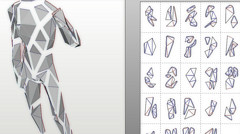
\includegraphics[scale=0.75]{images/test.jpg}
    \caption{The Toucan}
  \end{center}
\end{figure}

\chapter{ReadingList}

\hypertarget{related_readings_1}{}\subsection*{{Related readings}}\label{related_readings_1}

\href{http://dspace.mit.edu/handle/1721.1/33012}{New information technologies in the old political economy : an exploration of community-based GIS for improving basic services for the poor in New Delhi, India} - 2005 MIT DUSP dissertation by Claudia Canepa

\href{http://www.ejisdc.org/ojs2/index.php/ejisdc/article/viewFile/237/158}{PARTICIPATORY SPATIAL INFORMATION MANAGEMENT AND COMMUNICATION IN DEVELOPING COUNTRIES} - Giacomo Rambaldi, Peter A Kwaku Kyem, Mike $\backslash$McCall, Daniel Weiner, EJISDC, 2006

\href{http://books.google.com/books?id=4u79ffyzekoC&printsec=frontcover&dq=child%27s+pictorial+world&ei=5EUYS9veGqPqygShs7TVBw#v=onepage&q=&f=false}{The child'{}s creation of a pictorial world}, Claire Golomb

\href{http://www.unicef.org/teachers/researchers/intro.htm}{Curriculum on ``{}Children as Community Researchers''{}} - UNICEF, authored by \href{http://web.gc.cuny.edu/che/cerg/about_cerg/environmental_learning_index.htm}{Children'{}s Environment Research Group}

\href{http://www.directionsmag.com/article.php?article_id=2365&trv=1.}{Participatory GIS - A Paradigm Shift in Development?} - Jen Osha and Daniel Weiner, 2006

\href{http://www.iapad.org/pgis2005/}{Mapping for Change} - 2005 International Conference on Participatory Spatial Information Management and Communication

Weiner, D. and T. Harris, 2003. ''{}\href{http://www.rri.wvu.edu/pdffiles/gisweiner.pdf}{Community-Integrated GIS for Land Reform in South Africa}.''{} URISA Journal. 15(2): 61-73.

\href{http://www.maptogether.net/taxonomy/term/151}{PPGIS on MapTogether.net}

\href{http://books.google.com/books?hl=en&lr=&id=_VK-ABCKlVgC&oi=fnd&pg=PA3&dq=Nino+Bariola&ots=_r1wMwjiou&sig=TH0Gn1P27Xtsdq2Oc0Up5D6HLzg#v=onepage&q=Nino%20Bariola&f=false}{Bilingualism and identity: Spanish at the crossroads with other languages} - Geographic dispute in Canta Gallo, in Lima, \href{http://books.google.com/books?id=_VK-ABCKlVgC&lpg=PA3&ots=_r1wMwjiou&dq=Nino%20Bariola&lr=&pg=PA153#v=onepage&q=&f=true}{Chapter 7}

\href{http://www.sciencedirect.com/science?_ob=ArticleURL&_udi=B6VG2-4XHJX4B-1&_user=10&_coverDate=08/31/2009&_rdoc=1&_fmt=high&_orig=search&_sort=d&_docanchor=&view=c&_searchStrId=1186930669&_rerunOrigin=google&_acct=C000050221&_version=1&_urlVersion=0&_userid=10&md5=a9327ffa62e089e863f892a4551c1717}{Intervention: Mapping is critical!} - This intervention targets the much heralded demise of the map in geography and the recently proposed “rethinking” of maps. It comprises contributions from two political geographers, a military geographer, a political scientist, and two activist cartographers and argues that there is not so much a need to “rethink” maps, but to “re-engage” with the material practices of mapping, and above all to “re-make” maps.

\href{http://training.esri.com/campus/library/bibliography/RecordDetail.cfm?ID=95545&browseonly=0}{Mapping in a Shoebox} - A Grassroots Approach for Developing the Geospatial Literacy of Elementary Children - 24th International Cartographic Conference - Jaqueline M. Anderson, Sally Hermansen, Lorraine Innes, 2009

Lots of work by Proboscis: \href{http://urbantapestries.net/}{Social Tapestries/Urban Tapestries}, 2002-7 - Urban Tapestries investigated how, by combining mobile and internet technologies with geographic information systems, people could `{}author'{} the environment around them; a kind of Mass Observation for the 21st Century. Like the founders of Mass Observation in the 1930s, we were interested creating opportunities for an ``{}anthropology of ourselves''{} – adopting and adapting new and emerging technologies for creating and sharing everyday knowledge and experience; building up organic, collective memories that trace and embellish different kinds of relationships across places, time and communities.

\href{http://www.geoconnections.org/publications/Key_documents/Sensitive_Env_Geo_Data_Guide_EN_v1.pdf}{BEST PRACTICES FOR SHARING SENSITIVE ENVIRONMENTAL GEOSPATIAL DATA} - for GeoConnections by AMEC Earth \& Environmental, 2010



%%%%%%%%%%%%%%%%%%%%%%%%% BIBLIOGRAPHY
\nocite{*}
{\small
\bibliographystyle{plain}
\bibliography{thesis}
}

\end{document}
